\chapter{原理 \label{chap:principles}}
\section{深層学習 \label{section:deep-learning}}
深層学習は機械学習の一分野であり,複数の隠れ層から成るニューラルネットワークを使用して高度なパターン認識や特徴抽出を行う手法である\cite{doi:10.1126/science.1127647}.この章では最も単純で典型的な深層学習のアーキテクチャを説明する.
\if0
どのくらい書くべきか?どう書くべきか?
この原理の章はそもそも自分のモデルを説明するときに使うものであって,先に自分のモデルについて書いたほうがやりやすいかもしれん.
- 読者にどの程度の前提知識を求めるべきか.
\fi

図\ref{fig:dnn-architecture}に示す通り,深層学習は入力層,隠れ層,出力層から成るニューラルネットワークで表される.入力層は入力データを受け取り,隠れ層は入力層から出力を受け取り,出力層は隠れ層の出力を受け取る.隠れ層は複数存在し,それぞれの隠れ層は前の隠れ層の出力を受け取る.ここで,各層は複数のニューロンからなり,各ニューロンは入力された実数値に活性化関数を適用した値を出力する.図\ref{fig:dnn-architecture}中の破線矢印が活性化関数に対応する.そしてその入力値は,前の層のニューロンの出力に重みをかけたものの和にバイアスを加えた値である.これは図\ref{fig:dnn-architecture}中の実線矢印に対応する.十分な隠れ層を持ち,重みが適切に調節されたニューラルネットワークは任意の関数を近似することができることが知られている\cite{Hornik1989MultilayerFN}.

\begin{figure}[bp]
  \centering
  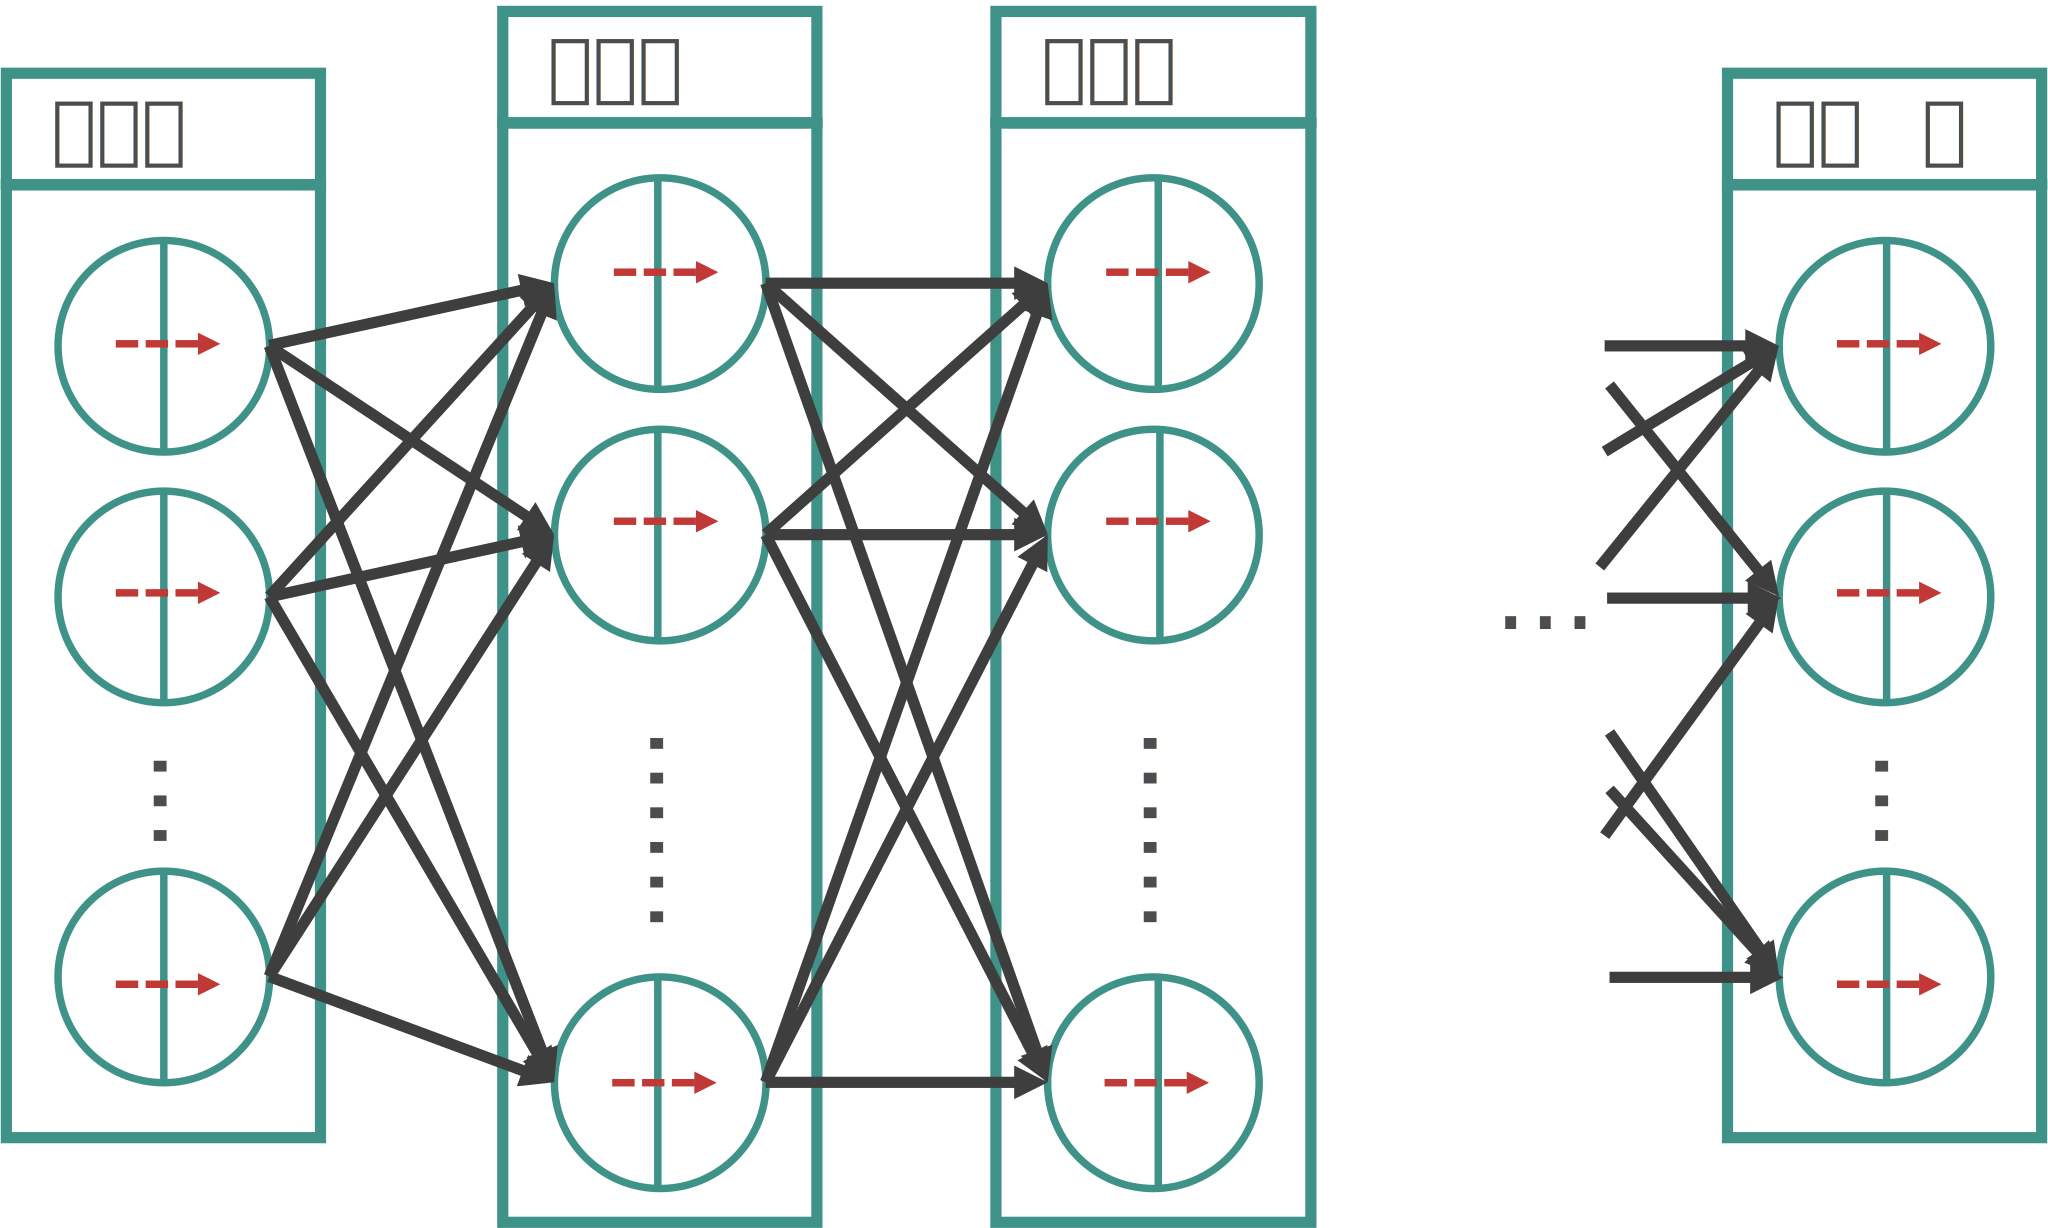
\includegraphics[width=0.7\linewidth]{./principles/figs/dnn_overview.svg.eps}
  \caption{深層学習のアーキテクチャ}
  \label{fig:dnn-architecture}
\end{figure}

\subsection{ニューラルネットワークの計算原理 \label{subsection:neuron-principles}}
より詳しく原理を説明する.合計で$m$層になるニューラルネットワークを考える.まず,入力層のニューロンの数を$n^{(1)}$とし,第$j$ ($1 \leq j \leq n^{(1)}$)ニューロンへの入力を$y_j^{(1)} \in \mathbb{R}$,ニューロンからの出力を$z_j^{(1)} \in \mathbb{R}$とする.$y_j^{(1)}$は入力データの第$j$成分を意味する.また,$z_j^{(1)}$は$y_j^{(1)}$に活性化関数$f^{(1)}: \mathbb{R} \rightarrow \mathbb{R}$を適用した値である.つまり,
\begin{equation}
  z_j^{(1)} = f^{(1)}(y_j^{(1)})
  \label{eq:deep-learning-input-layer}
\end{equation}
である.
次に,中間層または出力層である第$k$ $(2 \leq k \leq m)$層のニューロンの数を$n^{(k)}$とし,第$j$ $(1 \leq j \leq n^{(k)})$ニューロンへの入力を$y_j^{(k)} \in \mathbb{R}$,ニューロンからの出力を$z_j^{(k)} \in \mathbb{R}$とすると,これらは以下のように表される.
\begin{equation}
  y_j^{(k)} = \sum_{i=0}^{n^{(k-1)}} w_{ij}^{(k)} z_i^{(k-1)}
  \label{eq:deep-learning-neuron-input}
\end{equation}
\begin{equation}
  z_j^{(k)} = f^{(k)}(y_j^{(k)})
  \label{eq:deep-learning-neuron-output}
\end{equation}
ここで,$w_{ij}^{(k)} \in \mathbb{R}$は第$k-1$層の第$i$ニューロンから第$k$層の第$j$ニューロンへの重み,$f^{(k)}: \mathbb{R} \rightarrow \mathbb{R}$は活性化関数である.ただし,$f^{(m)}$は恒等関数とする.活性化関数は通常非線形関数であり,シグモイド関数やReLU関数などが用いられる.またここでは$z_0^{(k-1)} = 1$とすることで,バイアス$w_{0j}^{(k)}$を導入する.

以上から,ニューラルネットワークに$y_1^{(1)}, \dots, y_{n^{(1)}}^{(1)}$を入力すると式(\ref{eq:deep-learning-input-layer}), (\ref{eq:deep-learning-neuron-input}), (\ref{eq:deep-learning-neuron-output})
によって順次計算が行われ,$z_1^{(m)}, \dots, z_{n^{(m)}}^{(m)}$が出力されることがわかる.続いて,これをどのように目的の出力に近づけるかを考える.

目的の出力を$\hat{z}_0^{(m)}, \dots, \hat{z}_{n^{(m)}}^{(m)}$とする.このとき,出力層のニューロンの出力と目的の出力の誤差を表す二乗損失関数は次のように表される(これは単に損失とも呼ばれる).
\begin{equation}
  E = \frac{1}{2} \sum_{j=1}^{n^{(m)}} \left( z_j^{(m)} - \hat{z}_j^{(m)} \right)^2
  \label{eq:deep-learning-loss}
\end{equation}

これを最小化するように各層の重みを調節することで,ニューラルネットワークは目的の出力に近づく.ここでは最も単純な勾配降下法を用いる.まず,隠れ層及び出力層に接続する重み$w_{ij}^{(k)}$ $(2 \leq k \leq m)$の誤差$E$に対する勾配は$\partial E / \partial w_{ij}^{(k)}$で表され,これにより重みを次のように更新すると誤差が減少することが分かる.
\begin{equation}
  w_{ij}^{(k)} \leftarrow w_{ij}^{(k)} - \eta \frac{\partial E}{\partial w_{ij}^{(k)}}
  \label{eq:deep-learning-gradient-descent}
\end{equation}
ここで,$\eta$は学習率と呼ばれる$0$以上の実数である.以下では$\partial E / \partial w_{ij}^{(k)}$を求めることを考える.そのために準備としてひとつ記号を定義する.$\delta_j^{(k)}$を第$k$層の第$j$ニューロンの誤差といい,以下で定義する.
\begin{equation}
  \delta_j^{(k)} = \frac{\partial E}{\partial u_j^{(k)}}
  \label{eq:deep-learning-delta}
\end{equation}
これを用いて$\partial E / \partial w_{ij}^{(k)}$を表し,最後に誤差を求める.

$2 \leq k \leq m$とする.式(\ref{eq:deep-learning-neuron-output}), (\ref{eq:deep-learning-delta})より,$\partial E / \partial w_{ij}^{(k)}$は次のように表される.
\begin{equation}
  \frac{\partial E}{\partial w_{ij}^{(k)}} =
  \frac{\partial E}{\partial u_j^{(k)}} \frac{\partial u_j^{(k)}} {\partial w_{ij}^{(k)}} =
  \delta_j^{(k)} \frac{\partial u_j^{(k)}} {\partial w_{ij}^{(k)}}
  \label{eq:deep-learning-middle-layer}
\end{equation}
そして,式(\ref{eq:deep-learning-neuron-input})より,$\partial u_j^{(k)} / \partial w_{ij}^{(k)}$は次のように表される.
\begin{equation}
  \frac{\partial u_j^{(k)}} {\partial w_{ij}^{(k)}} =
  \frac{ \partial \left( \sum_{i=0}^{n^{(k-1)}} w_{ij}^{(k)} z_i^{(k-1)} \right)} {\partial w_{ij}^{(k)}} =
  z_i^{(k-1)}
  \label{eq:deep-learning-middle-layer-2}
\end{equation}
したがって,式(\ref{eq:deep-learning-middle-layer}), (\ref{eq:deep-learning-middle-layer-2})より,
\begin{equation}
  \frac{\partial E}{\partial w_{ij}^{(k)}} =
  \delta_j^{(k)} z_i^{(k-1)}
  \label{eq:deep-learning-middle-layer-3}
\end{equation}
となる.

最後に誤差を求める.まず,出力層の誤差$\delta_j^{(m)}$は式(\ref{eq:deep-learning-delta}), (\ref{eq:deep-learning-loss})より次のように表される.
\begin{equation}
  \delta_j^{(m)} = \frac{\partial E}{\partial u_j^{(m)}} =
  \frac{\partial E}{\partial z_j^{(m)}} =
  \frac{\partial \left( \frac{1}{2} \sum_{j=1}^{n^{(m)}} \left( z_j^{(m)} - \hat{z}_j^{(m)} \right)^2 \right)} {\partial z_j^{(m)}} =
  z_j^{(m)} - \hat{z}_j^{(m)}
  \label{eq:deep-learning-output-error}
\end{equation}
続いて,$2 \leq k \leq m-1$に対して,第$k$層の誤差$\delta_j^{(k)}$は次のように表される.
\begin{equation}
  \begin{split}
  \delta_j^{(k)} &= \frac{\partial E}{\partial u_j^{(k)}} =
  \sum_{i=1}^{n^{(k+1)}} \frac{\partial E}{\partial u_i^{(k+1)}} \frac{\partial u_i^{(k+1)}} {\partial u_j^{(k)}} \\ &=
  \sum_{i=1}^{n^{(k+1)}} \delta_i^{(k+1)} \frac{\partial u_i^{(k+1)}} {\partial z_j^{(k)}} \frac{\partial z_j^{(k)}} {\partial u_j^{(k)}} \\ &=
  \sum_{i=1}^{n^{(k+1)}} \delta_i^{(k+1)} w_{ji}^{(k+1)} f^{(k)\prime}(y_j^{(k)})
  \end{split}
  \label{eq:deep-learning-middle-error}
\end{equation}

以上より,式(\ref{eq:deep-learning-output-error}), (\ref{eq:deep-learning-middle-error})を用いて$\delta_j^{(k)}$を順次計算し,さらに式(\ref{eq:deep-learning-middle-layer-3})を用いて$\partial E / \partial w_{ij}^{(k)}$を順次計算することで,式(\ref{eq:deep-learning-gradient-descent})によって重みを更新することができる.

\subsection{自動微分 \label{subsection:automatic-differentiation}}
\ref{subsection:neuron-principles}項では,ニューラルネットワークの重みを更新するために誤差を逐次的に求めていく必要があることを述べた.しかし,ニューラルネットワークのモデルが複雑化するに従ってこの数式を手作業で計算することは困難になってくる.そこで,自動微分と呼ばれる手法を用いる.
一般的にコンピュータ上で表される関数は,基本的には四則演算や三角関数,指数関数などの初等関数の合成で表される\cite{10.5555/3122009.3242010}.自動微分では,このような基本的な関数の微分をあらかじめ定義しておき,合成関数の微分を関数の微分の積で表すことで計算する\cite{10.5555/3122009.3242010}.PyTorch\cite{NEURIPS2019-9015}やTensorFlow\cite{tensorflow2015-whitepaper}などの深層学習フレームワークでは,この自動微分が実装されているため複雑なモデルでも容易に実装することができる.

\section{格子ボルツマン法 \label{section:lbm}}

格子ボルツマン法(LBM, Lattice Boltzmann Method)は数値流体力学の一手法である.流体を有限種類の速度を持つ仮想粒子の集合とみなし,その分布関数を時空間で離散化したものに対して並進と衝突と呼ばれる操作を逐次施すことで流体の動きを表現する\cite{doi:10.1146/annurev.fluid.30.1.329}.この章では,LBMの基本的な原理を説明する.

等温場の格子流体モデルとして,ここではD2Q9モデルを考える.D2Q9モデルは,仮想粒子の速度ベクトルが以下の式に示す9種類である二次元空間格子モデルである.
\begin{equation}
  \bm{v} = \left( \pm 1, \pm 1 \right), \left( \pm 1, 0 \right), \left( 0, \pm 1 \right), \left( 0, 0 \right)
  \label{eq:lbm-velocity}
\end{equation}
ただし,複号任意である.これは図\ref{fig:d2q9}に示すとおり,速度ベクトルは格子の中心からのオフセットで表されることを意味している.この下で,分布関数$f(\bm{x}, \bm{v}, t)$は無次元座標$\bm{x} \in \mathbb{R}^2$,無次元時刻$t \in \mathbb{R}$における速度$\bm{v}$の粒子数を表す.すると,これは任意の$\bm{v}$について以下の離散ボルツマン方程式に従う\cite{Inamuro1990NumericalSO}.
\begin{equation}
  \mathrm{Sh} \frac{\partial f(\bm{x}, \bm{v}, t)}{\partial t} + \bm{v} \cdot \nabla f(\bm{x}, \bm{v}, t) = \frac{1}{\epsilon} \Omega_{\bm{v}}\left[ f(\bm{x}, \bm{v}', t) \right]
  \label{eq:lbm-discrete-boltzmann}
\end{equation}
\begin{figure}[bp]
  \centering
  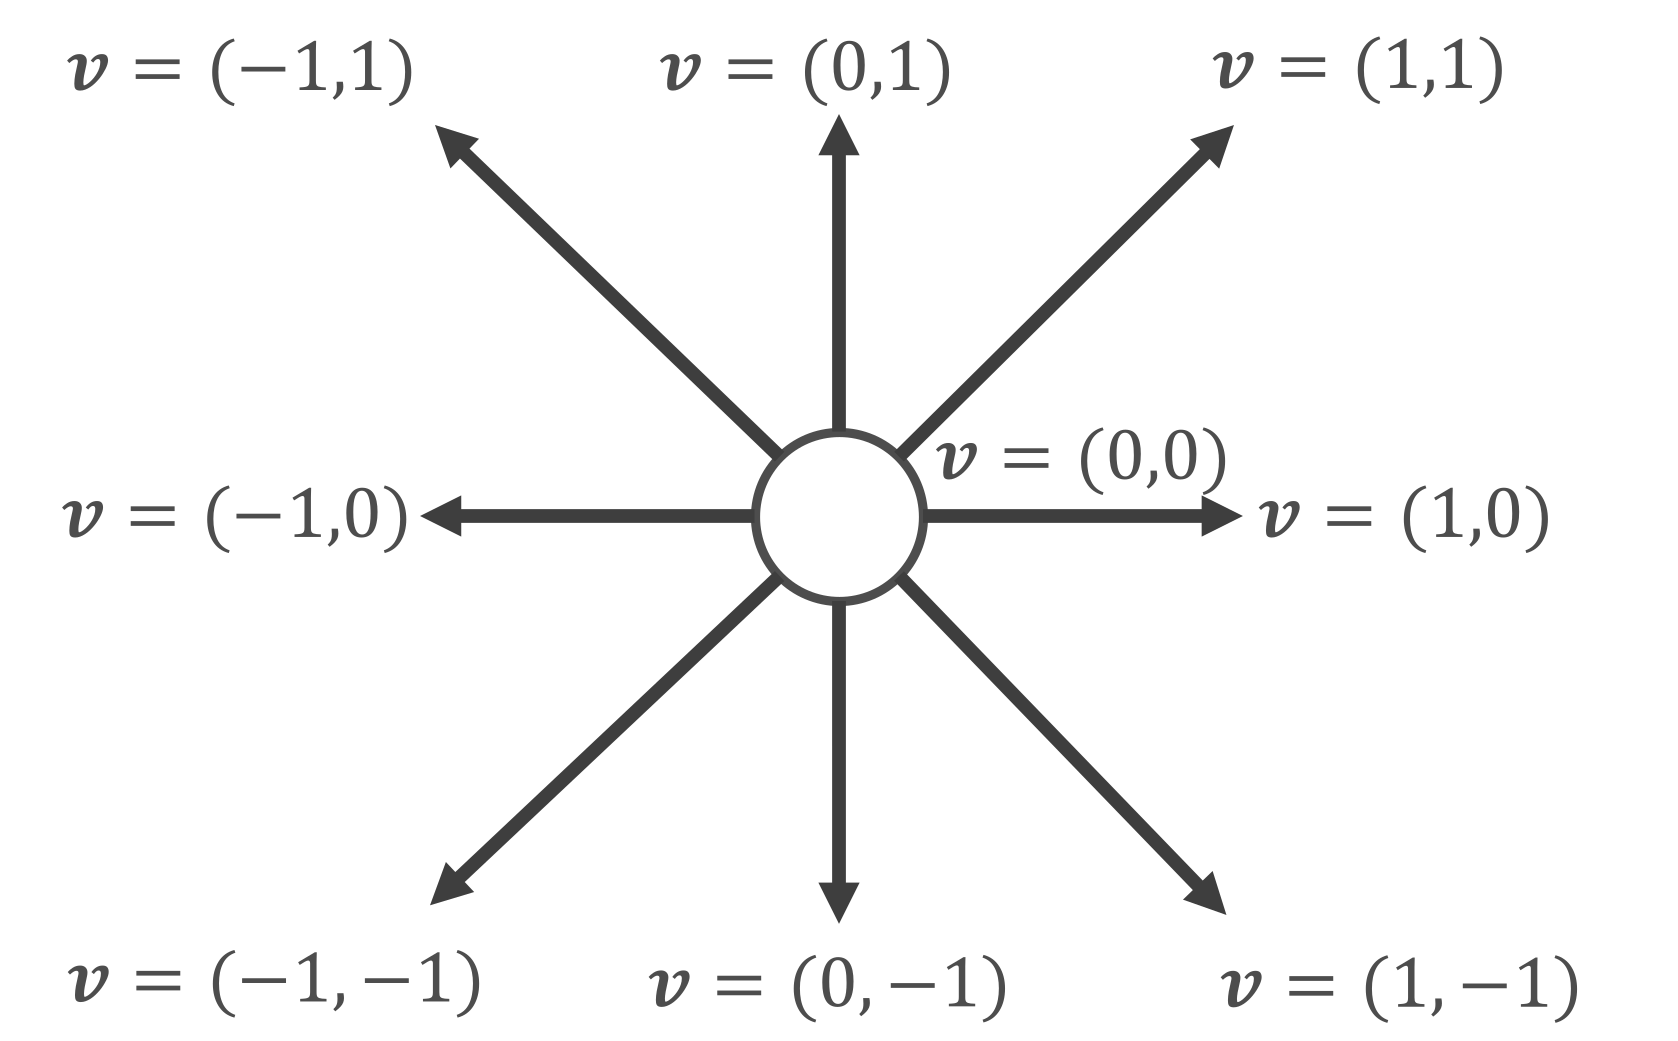
\includegraphics[width=0.6\linewidth]{./principles/figs/lbm_d2q9.svg.eps}
  \caption{D2Q9モデルの速度ベクトル}
  \label{fig:d2q9}
\end{figure}
ここで,$\mathrm{Sh}$はストローハル数,$\epsilon$はクヌーセン数,$\Omega_{\bm{v}}$は仮想粒子の衝突による増減を表す衝突演算子である.ただし,$\bm{v}'$はパラメータ化されておりすべての$\bm{v}'$について演算を行うと約束する.続いて,空間と時間を$\Delta x = 1/\epsilon$, $\Delta t = \mathrm{Sh} \Delta x$によってそれぞれ分割し,式(\ref{eq:lbm-discrete-boltzmann})を時空間について一次前進差分によって近似すると次式を得る.
\begin{equation}
  f(\bm{x}+\bm{v}\Delta t, \bm{v}, t+\Delta t) - f(\bm{x}, \bm{v}, t) = \Omega_{\bm{v}}\left[ f(\bm{x}, \bm{v}', t) \right]
  \label{eq:lbm-lattice-boltzmann}
\end{equation}
また,離散化された時空間上での分布関数から,流体の巨視的な密度$\rho(\bm{x}, t)$と巨視的な流速$\bm{u}(\bm{x}, t)$は以下のように定義される.
\begin{equation}
  \rho(\bm{x}, t) = \sum_{\bm{v}} f(\bm{x}, \bm{v}, t)
  \label{eq:lbm-macro-density}
\end{equation}
\begin{equation}
  \rho(\bm{x}, t) \bm{u}(\bm{x}, t) = \sum_{\bm{v}} \bm{v} f(\bm{x}, \bm{v}, t)
  \label{eq:lbm-macro-velocity}
\end{equation}
式(\ref{eq:lbm-lattice-boltzmann})において,左辺が並進,右辺が衝突を表していることに注意されたい.この右辺に次式で表されるBGK(Bhatnagar-Gross-Krook)モデルと呼ばれる衝突演算子\cite{PhysRev.94.511}を導入する.
\begin{equation}
  \Omega_{\bm{v}}\left[ f(\bm{x}, \bm{v}', t) \right] = -\frac{1}{\tau} \left[ f(\bm{x}, \bm{v}, t) - f^{eq}(\bm{x}, \bm{v}, t) \right]
  \label{eq:lbm-bgk}
\end{equation}
ここで,$\tau$は流体の無次元緩和時間,$f^{eq}(\bm{x}, \bm{v}, t)$は局所平衡分布関数と呼ばれる関数である.式(\ref{eq:lbm-bgk})を式(\ref{eq:lbm-lattice-boltzmann})に代入すると,次式を得る.
\begin{equation}
  f(\bm{x}+\bm{v}\Delta t, \bm{v}, t+\Delta t) = f(\bm{x}, \bm{v}, t) - \frac{1}{\tau} \left[ f(\bm{x}, \bm{v}, t) - f^{eq}(\bm{x}, \bm{v}, t) \right]
  \label{eq:lbm-bgk-lattice-boltzmann}
\end{equation}
最後に,局所平衡分布関数を求める.この関数は
\begin{equation}
  \rho(\bm{x}, t) = \sum_{\bm{v}} f^{eq}(\bm{x}, \bm{v}, t)
  \label{eq:lbm-eq-macro-density}
\end{equation}
\begin{equation}
  \rho(\bm{x}, t) \bm{u}(\bm{x}, t) = \sum_{\bm{v}} \bm{v} f^{eq}(\bm{x}, \bm{v}, t)
  \label{eq:lbm-eq-macro-velocity}
\end{equation}
を満たす必要がある.これらを満たす局所平衡分布関数はマクスウェル分布\cite{Asakura1989}において$|\bm{u}|$が二次の項まで展開すると得られて,以下のように定義される.
\begin{equation}
  f^{eq}(\bm{x}, \bm{v}, t) = c(\bm{v}) \rho(\bm{x}, t) \left[ 1 + 3\bm{v} \cdot \bm{u}(\bm{x}, t) + \frac{9}{2}(\bm{v} \cdot \bm{u}(\bm{x}, t))^2 - \frac{3}{2}\bm{u}(\bm{x}, t)^2 \right]
  \label{eq:lbm-eq-1}
\end{equation}
ただし,式(\ref{eq:lbm-eq-macro-density}), (\ref{eq:lbm-eq-macro-velocity}), (\ref{eq:lbm-eq-1})内の$\rho(\bm{x}, t)$, $\bm{u}(\bm{x}, t)$はそれぞれ式(\ref{eq:lbm-macro-density}), (\ref{eq:lbm-macro-velocity})で求めた値を用いる.また,$c(\bm{v})$は速度ベクトル$\bm{v}$に対する重みであり,D2Q9モデルでは
\begin{equation}
  c(\bm{v}) = \left\{
    \begin{array}{ll}
      4/9 & (\bm{v} = (0, 0)) \\
      1/9 & (\bm{v} = (\pm 1, 0), (0, \pm 1)) \\
      1/36 & (\bm{v} = (\pm 1, \pm 1))
    \end{array}
  \right.
  \label{eq:lbm-weight}
\end{equation}
と求められる.以上の式(\ref{eq:lbm-bgk-lattice-boltzmann}), (\ref{eq:lbm-eq-1}), (\ref{eq:lbm-macro-density}), 及び(\ref{eq:lbm-macro-velocity})によりLBMの基本的な計算スキームが構成された.これらの計算スキームはChapman-Enskog展開によってナビエ・ストークス方程式を空間二次精度で再現することが知られている\cite{Inamuro2020}.

本研究においては時空間間隔をリスケールし,$\Delta x = 1$, $\Delta t = 1$として計算を行った.その上で式(\ref{eq:lbm-bgk-lattice-boltzmann})は次のように並進と衝突の式に分離することができる.
\begin{equation}
  f'(\bm{x}+\bm{v}, \bm{v}, t)
  = f(\bm{x}, \bm{v}, t)
  \label{eq:lbm-streaming}
\end{equation}
\begin{equation}
  f(\bm{x}, \bm{v}, t+1)
  = f'(\bm{x}, \bm{v}, t) - \frac{1}{\tau} \left[ f'(\bm{x}, \bm{v}, t) - f^{eq}(\bm{x}, \bm{v}, t) \right]
  \label{eq:lbm-collision}
\end{equation}
このとき,式(\ref{eq:lbm-eq-1})は次のように表される.
\begin{equation}
  f^{eq}(\bm{x}, \bm{v}, t) = c_i(\bm{v}) \rho'(\bm{x}, t) \left[ 1 + 3\bm{v} \cdot \bm{u}'(\bm{x}, t) + \frac{9}{2}(\bm{v} \cdot \bm{u}'(\bm{x}, t))^2 - \frac{3}{2}\bm{u}'(\bm{x}, t)^2 \right]
  \label{eq:lbm-eq}
\end{equation}

